\documentclass[tikz,border=3pt]{standalone}
\usepackage[utf8]{inputenc}
\usepackage[T1]{fontenc}
\usepackage{libertinus}
\usepackage{amsmath,amssymb}
\usetikzlibrary{arrows.meta,calc,patterns,decorations.pathmorphing,decorations.markings,decorations.pathreplacing,bending}
\definecolor{UGblue}{RGB}{0,51,102}
\newcommand{\dbar}{\mathchar'26\mkern-12mu d}
\tikzset{
  >=Stealth,
  every node/.style={font=\small},
  caja/.style={draw,line width=0.9pt},
  pared/.style={draw,line width=1.6pt},
  ejes/.style={->,line width=0.8pt},
  adia/.style={draw,pattern=north east lines,pattern color=black!70,line width=0.5pt},
  gas/.style={fill=UGblue!8},
  punto/.style={fill,circle,inner sep=1.3pt},
  onda/.style={decorate,decoration={snake,amplitude=1.1pt,segment length=5pt,post length=3pt,pre length=0pt}},
}
\begin{document}
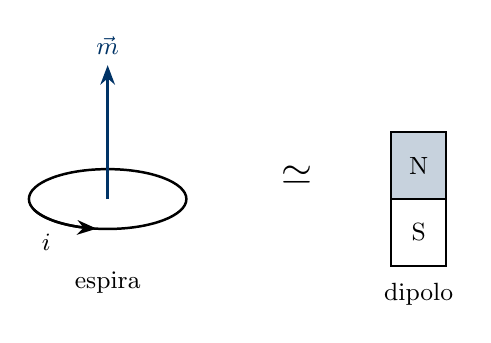
\begin{tikzpicture}
  \draw[line width=0.9pt] (0,0) ellipse (1.0 and 0.38);
  \draw[->,line width=0.9pt] plot[domain=200:262] ({1.0*cos(\x)},{0.38*sin(\x)});
  \node[below left] at (-0.6,-0.32) {$i$};
  \draw[->,line width=0.9pt,UGblue] (0,0) -- (0,1.7) node[above] {$\vec m$};
  \node[below] at (0,-0.8) {espira};
  \node at (2.4,0.3) {\Large $\simeq$};
  \draw[line width=0.9pt] (3.6,-0.85) rectangle (4.3,0.85);
  \draw[line width=0.9pt] (3.6,0) -- (4.3,0);
  \fill[UGblue!22] (3.6,0) rectangle (4.3,0.85);
  \draw[line width=0.9pt] (3.6,-0.85) rectangle (4.3,0.85);
  \draw[line width=0.9pt] (3.6,0) -- (4.3,0);
  \node at (3.95,0.42) {N}; \node at (3.95,-0.42) {S};
  \node[below] at (3.95,-0.95) {dipolo};
\end{tikzpicture}
\end{document}
